% DO NOT COMPILE THIS FILE DIRECTLY!
% This is included by the other .tex files.

\begin{frame}[t,plain]
\titlepage
\end{frame}

\begin{frame}
 \frametitle{Origins}
 \begin{itemize}
         \item As the pandemic started we all quickly faced a set of new issues to tackle
         \begin{itemize}
              \item Remote work exposed completely {\bf new attack surfaces}
              \item We were all personally invested in {\bf tracking the evolution of the pandemic} itself
              \item There was a rampant {\bf abuse of the general chaos}, for a host of objectives
         \end{itemize}
         \item We saw more and more disjointed information popping up in our regular communities...
         \item ...but both the {\bf reach} and the {\bf interest} was varied
 \end{itemize}
\end{frame}

\begin{frame}
 \frametitle{COVID-19 MISP}
 \begin{itemize}
         \item COVID-19 MISP is a MISP instance retrofitted for COVID-19 info sharing
         \item We are focusing on three areas of sharing:
         \begin{itemize}
              \item {\bf Medical} information
              \item {\bf Cyber threats} related to / abusing COVID-19
              \item {\bf Disinformation} related to COVID-19
         \end{itemize}
         \item Low barrier of entry, aiming for wide spread
         \item Has grown to become a {\bf massive community}
 \end{itemize}
\end{frame}

\begin{frame}
 \frametitle{Why?}
 \begin{itemize}
         \item We are obviously interested on a personal level, as is everyone
         \item {\bf Information sharing is what we do anyway}
         \item The idea was also to {\bf build tools that are reusable} for our more regular use-cases
         \item Bridging different domains affected in different ways can reveal {\bf correlations}
 \end{itemize}
\end{frame}

\begin{frame}
 \frametitle{Who did we consider to be the target audience?}
 \begin{itemize}
         \item Anyone wanting to gain {\bf situational awareness} for the current situation
         \item Security practicioners trying to fend off {\bf covid related attacks}
         \item Those wanting to share, collaborate, visualise, automate data
         \item All data is contextualised as {\bf either medical, security, disinformation or political} for easy filtering
 \end{itemize}
\end{frame}


\begin{frame}
 \frametitle{Customising MISP}
 \begin{itemize}
         \item We also wanted to sanity check ourselves, is MISP really flexible enough? Are we?
         \item We've set out a set of objectives that we wanted to achieve
         \begin{itemize}
              \item We wanted to be able to {\bf collect and track the spread of the pandemic}
              \item Also to be able to {\bf visualise} it in a meaningful way (this was early days for the pandemic)
              \item We wanted to {\bf rapidly ramp up a low barrier-of entry community}
              \item Ensure that the different topics of sharing can co-exist
         \end{itemize}
         \item We've quickly realised that we would need to modify MISP to make it work
 \end{itemize}
\end{frame}

\begin{frame}
 \frametitle{The initial plan}
 \begin{itemize}
         \item Find a good {\bf source of health information} - We chose John Hopkins, Chinese governmental data
         \item Build {\bf data models} to support it and integration tools
         \item MISP was lacking a built-in, distributed and ACL aware way of visualise data - {\bf new dahsboard}
         \item {\bf User enrollment} was painful at scale, we needed something simpler to tackle this
 \end{itemize}
\end{frame}

\begin{frame}
    \frametitle{Modelling new data structures for COVID-19}
    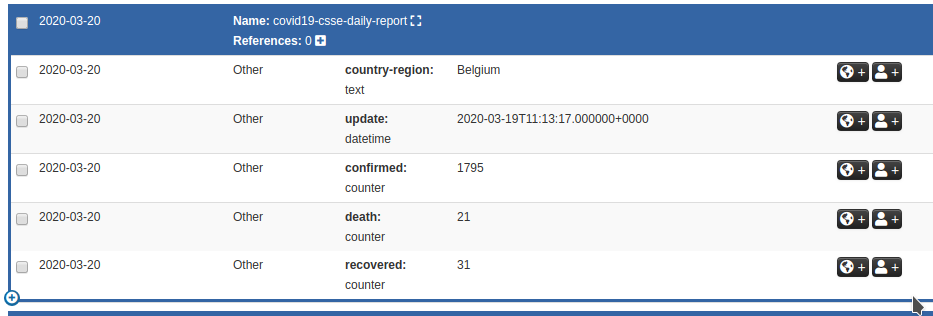
\includegraphics[width=1.00\linewidth]{covidobject.png}
    Mapping the data model was a simple task in itself
\end{frame}

\begin{frame}
    \frametitle{We've built ingestion scripts for the data-sets}
    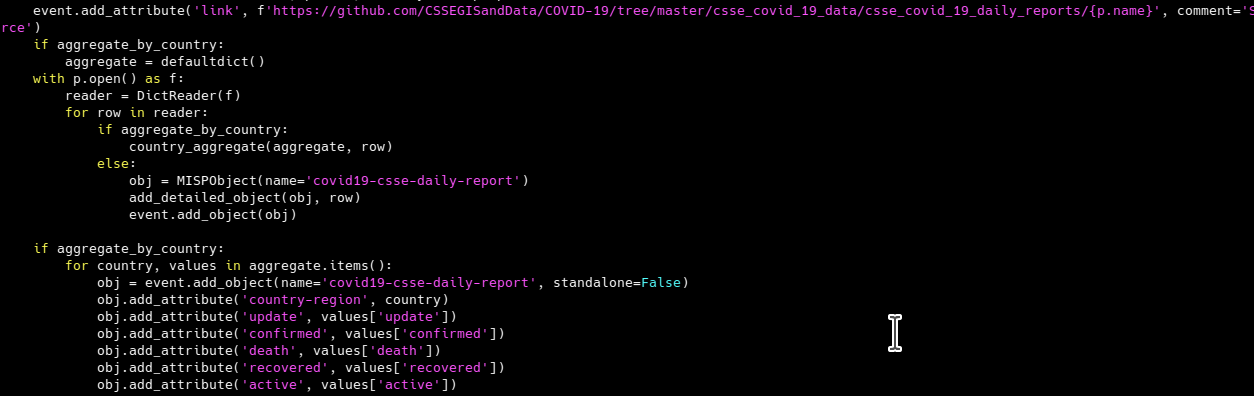
\includegraphics[width=1.00\linewidth]{johnhopkins.png}
    \url{https://github.com/MISP/PyMISP/tree/main/examples/covid19}
\end{frame}

\begin{frame}
    \frametitle{Strategy}
 \begin{itemize}
         \item Create {\bf daily events} for each source
         \item One object per country/region, with the appropriate numbers encoded
         \item Allows for easy data-range based searches and aggregation
         \item We ran into several issues to work around (inconsistent country names over time, count corrections, etc)
 \end{itemize}
\end{frame}

\begin{frame}
    \frametitle{Baseline information}
 \begin{itemize}
         \item In order to make sense of the data we needed {\bf population information}
         \item New {\bf country galaxy} with population counts
         \item Population numbers are not that easy to get ahold of in a standardised, machine parsable way...
 \end{itemize}
\end{frame}

\begin{frame}
    \frametitle{Designing a new dashboard system}
 \begin{itemize}
         \item Now we've had all this data in MISP, but how can we make sense of it?
         \item We wanted a new dashboard system
         \begin{itemize}
              \item It should {\bf adhere to ACL} rules of the data-set
              \item {\bf Easy to modify}, we didn't want this to be a one-off
              \item {\bf Customisable by the users} (we were all interested in different data, regions)
              \item But we still wanted to be able to {\bf provide baselines} for users so they don't have to fiddle with it
         \end{itemize}
         \item This and the parsing of the data were probably the two most demanding tools we had to build
 \end{itemize}
\end{frame}

\begin{frame}
    \frametitle{Dashboard}
    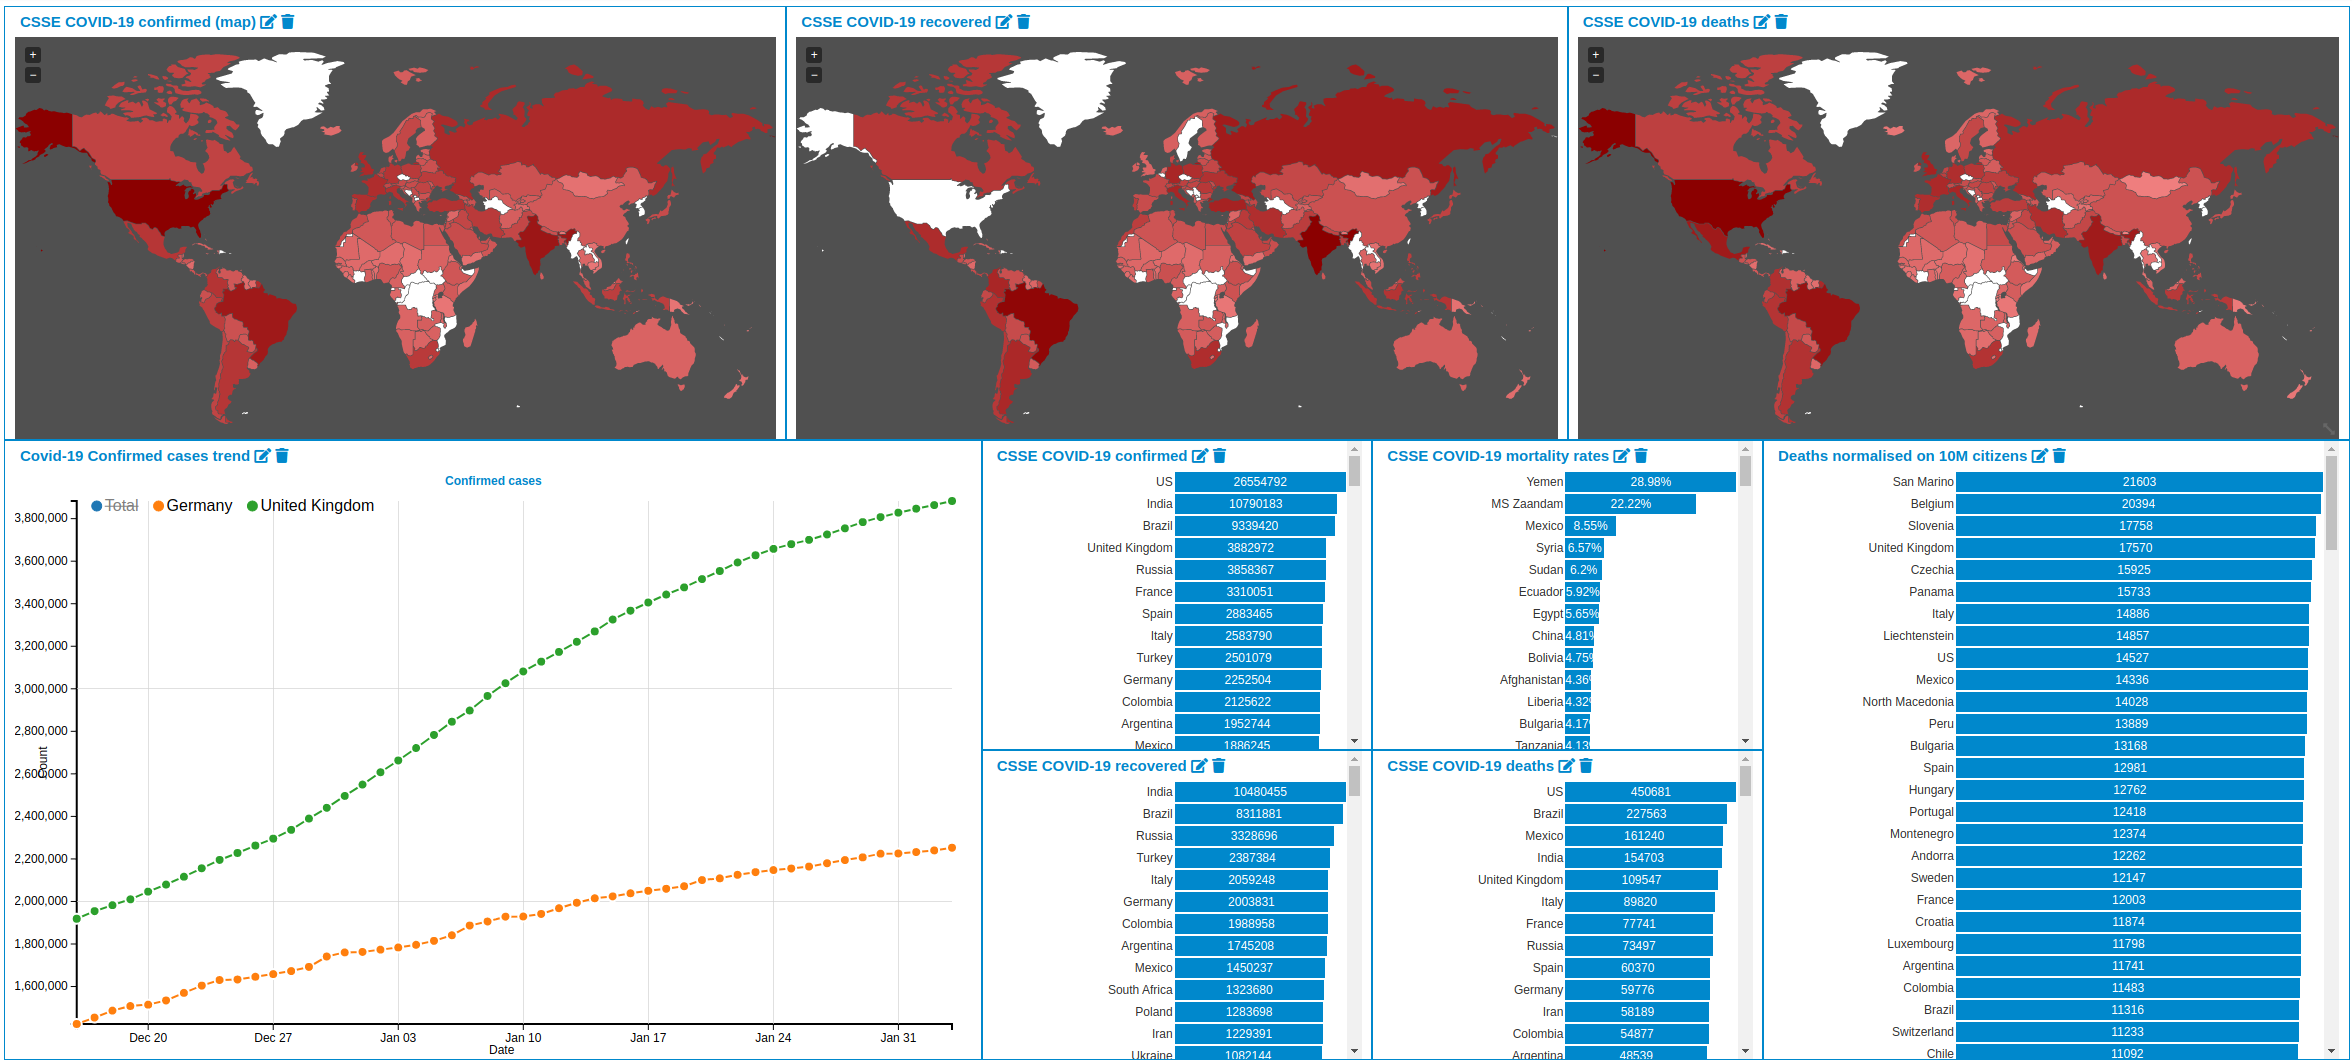
\includegraphics[width=1.00\linewidth]{covid-dashboard.png}
\end{frame}

\begin{frame}
    \frametitle{User management}
 \begin{itemize}
         \item We were getting hammered with ~50 user registrations per day at the start
         \item User registrations were a dialogue and time intensive
         \item The solution was a self registration system
         \begin{itemize}
              \item Users could ask for access with their contact information
              \item It was possible to encode MISP organisations in the request
              \item Users could indicate the level of access they wanted
         \end{itemize}
 \end{itemize}
\end{frame}

\begin{frame}
    \frametitle{Registration}
    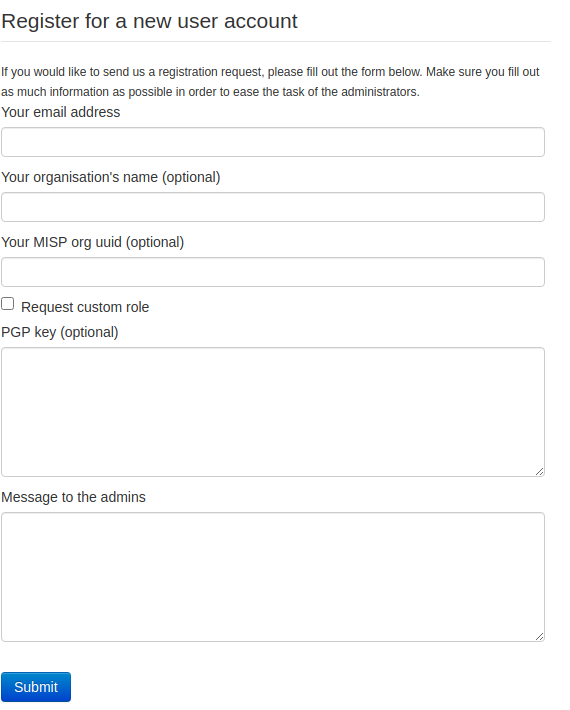
\includegraphics[width=0.50\linewidth]{registration1.png}
    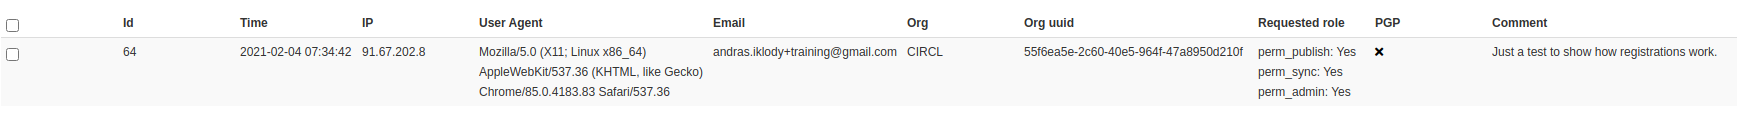
\includegraphics[width=1.00\linewidth]{registration2.png}
\end{frame}

\begin{frame}
    \frametitle{Filtering}
    \begin{itemize}
         \item We were getting hammered with ~50 user registrations per day at the start
    \end{itemize}
    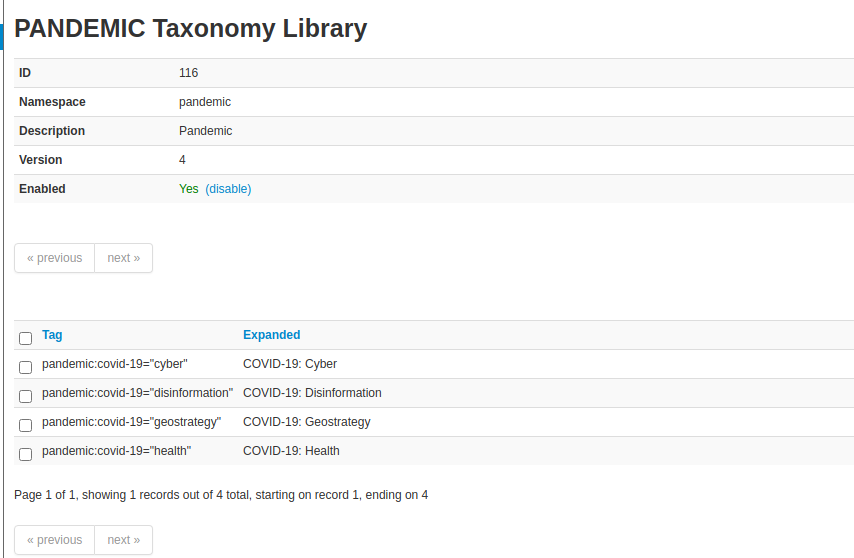
\includegraphics[width=0.80\linewidth]{taxonomy.png}
\end{frame}

\begin{frame}
    \frametitle{Feeds}
 \begin{itemize}
         \item Several feeds emerged from the community to tackle covid related threats
         \item Some of the feeds became warninglists to avoid blocking legitimate, national COVID-19 initiatives
         \item CTI league, Krassimir's whitelist, etc
         \item Integrating them was no effort though luckily
 \end{itemize}
\end{frame}

\begin{frame}
    \frametitle{So how much did all of this take?}
 \begin{itemize}
         \item One long weekend and a few extra days of development
         \item Most of the effort went into refining the data-sets, rules, etc of the community
         \item We had to deal with some level of abuse during the past year as well
         \item One of the biggest hurdles was possibly internal resistence against the project
 \end{itemize}
\end{frame}


\begin{frame}
\frametitle{How can you get involved?}
    \begin{itemize}
        \item Join the COVID-19 community
        \item Either just use the data, or contribute data back, examples:
        \begin{itemize}
            \item Ongoing Covid-19 phishing campaigns
            \item Sharing warninglists of known valid covid-19 related websites
            \item Local articles about the situation in your area
            \item Best practice recommendations
            \item Informations on travel restrictions
        \end{itemize}
        \item Create {\bf pull requests}
        \item Share your ideas
    \end{itemize}
\end{frame}

\begin{frame}
  \frametitle{Contact us}
  \begin{itemize}
    \item \url{https://www.misp-project.org/}
    \item \url{https://www.misp-standard.org/}
    \item \url{https://github.com/MISP}
    \item \url{info@misp-project.org}
    \item \url{https://twitter.com/MISPProject}
  \end{itemize}
\end{frame}


